\documentclass{article}
\usepackage{fixltx2e}
\usepackage[utf8]{inputenc}

\begin{document}

% Titelsida -----------------------------
\begin{titlepage}
\begin{center}

% Upper part of the page. The '~' is needed because \\
% only works if a paragraph has started.

\textsc{\LARGE Link{\"o}pings Universitet}\\[1.5cm]


% Title
{ \huge \bfseries Modellbaserad reglering av dubbeltankar \\[0.4cm] }

% Author and supervisor
\large
\emph{Av:}\\
Hans-Filip \textsc{Elo} och Niklas \textsc{Ericson}

\vfill

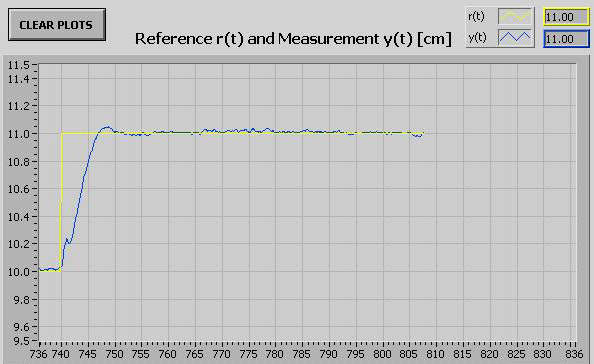
\includegraphics[scale=1, angle=0]{Test3_cut.jpg}

% Bottom of the page
{\large \today}

\end{center}
\end{titlepage}

% Slut på titelsida. ---------------------

\section{Inledning}
Detta {\"a}r en laborationsrapport p{\aa} reglersystem av pumpen till inloppet för tv{\aa} vattentankar med sammankopplade ut - och inlopp. Systemet skissas nedan i figur 1. 

\subsection{Syfte}
Att framst{\"a}lla en modell för automatisk reglering av {\"o}nskad vattenniv{\aa} i den undre tanken. 

\section{Metod}


\subsection{Materiel}

\section{Resultat}

\section{Slutsats}

\end{document}